\subsubsection{Sequence Diagrams}
	Some sequence diagrams of the system's most interesting aspects
	\begin{center}
		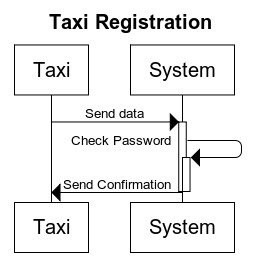
\includegraphics[width=0.60\textwidth]{./images/Taxi_Registration}
	\end{center}
	In order to register a taxi must send his identifier and a password to the system that localize him using the gps and inserts him into the appropriate queue. After this the system confirms the registration.
		\newpage
	\begin{center}
		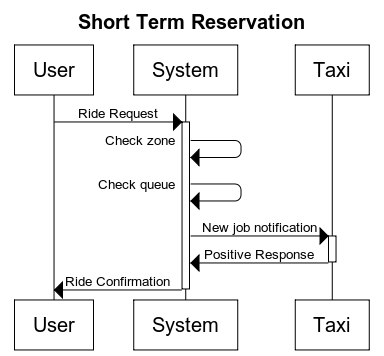
\includegraphics[width=0.80\textwidth]{./images/Short_Term_Reservation}
	\end{center}
	In order to request a short term reservation ride a user must send his address; date and hours must be omitted in this case. The system check where the address is located and the queue associated to that zone; then sends a notification to the first taxi in the queue and after the taxi confirmation, the system confirms the reservation to the user.
		\newpage
	\begin{center}
		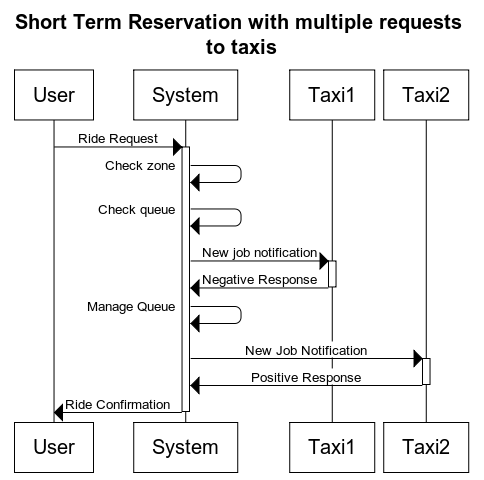
\includegraphics[width=0.90\textwidth]{./images/Short_Term_Reservation_with_multiple_requests_to_taxis}
	\end{center}
	In order to request a short term reservation ride a user must send his address; date and hours must be omitted in this case. The system check where the address is located and the queue associated to that zone; then sends a notification to the first taxi in the queue and since the first taxi answers with a negative response the system puts the taxi at the end of the queue and asks to the second taxi in the queue. After the taxi confirmation, the system confirms the reservation to the user.
		\newpage
	\begin{center}
		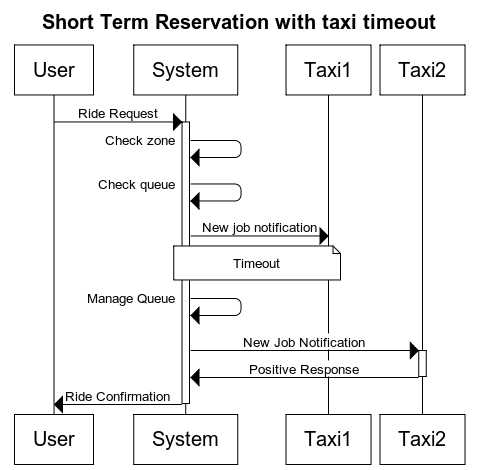
\includegraphics[width=0.90\textwidth]{./images/Short_Term_Reservation_with_taxi_timeout}
	\end{center}
	In order to request a short term reservation ride a user must send his address; date and hours must be omitted in this case. The system check where the address is located and the queue associated to that zone; then sends a notification to the first taxi in the queue and since the first taxi doesn't answers the system, after a timeout, puts the taxi at the end of the queue and asks to the second taxi in the queue. After the taxi confirmation, the system confirms the reservation to the user.
		\newpage
	\begin{center}
		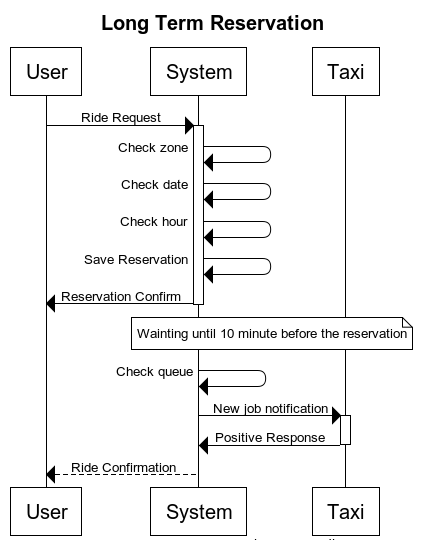
\includegraphics[width=0.90\textwidth]{./images/Long_Term_Reservation}
	\end{center}
	In order to request a long term reservation ride a user must send his address, the date and the hours of the reservation. Te system check where the address is located and stores the reservation i the database and confirms the user his reservation. Ten minutes before the ride the system check the queue associated with the address zone and send a notification to the taxi. After the positive answer by the taxi the system confirms the user his ride.
